% Provenance (never printed): see sources/outline_sources.md (Year 3: elastic waves
% recalled from the physics books; rays in a spherical Earth; travel-time tables;
% surface waves and dispersion; normal modes, told; linear inverse problems and
% seismic tomography). Brief: sources/book5/BRIEFS.md, ch. 1. Curves from
% figdata/bachelor-3/ray_tracing.py, love_dispersion.py, tomo_checkerboard.py;
% exercise and problem values in the Book 5 scratch calculator calc/ch01.py.
\chapter{Sismologia e imageamento da Terra}\label{ch:b3:seismology-imaging}

Em 22 de maio de 1960, às 19h11 do tempo universal, o maior terremoto registrado desde
1900 rompeu a zona de subducção ao largo do sul do Chile, com magnitude de 9.5.
% ledger: usgs5:chile1960
Suas ondas P chegaram a estações do outro lado do planeta cerca de vinte minutos
depois; suas ondas de superfície deram a volta ao globo várias vezes; e por dias
depois, os sismômetros de período longo registraram a Terra inteira vibrando com
períodos próximos de uma hora, como um sino golpeado. Cada um desses sinais carrega
informação sobre as rochas que atravessou. A partir dos tempos de chegada de milhões
dessas ondas, registradas em milhares de estações, os sismólogos construíram não apenas
o modelo estratificado da Terra recordado adiante, mas também imagens tridimensionais do
manto, nas quais as lajes que afundam e as plumas que sobem aparecem como regiões em que
as ondas se propagam um pouco mais rápido ou mais devagar que a média. Este capítulo mostra como:
como os raios se propagam numa Terra esférica, como as ondas de superfície sondam a crosta
e o manto por meio de sua dispersão, como as oscilações livres de todo o
planeta são descritas, e como alguns milhares de tempos de percurso são transformados em uma
imagem pela resolução de um \omterm{def:b3:seismology-imaging:inverse}{problema inverso} linear.

\begin{recall}
Em um sólido elástico isótropo propagam-se dois tipos de ondas de corpo: as ondas P, com a
velocidade $\alpha = \sqrt{(K + \tfrac43\mu)/\rho}$, e as ondas S, com
$\beta = \sqrt{\mu/\rho}$, onde $K$ e $\mu$ são os módulos de compressão e de cisalhamento
e $\rho$ a densidade; ondas S não atravessam um líquido (o volume do terceiro ano dos
livros de física, no capítulo sobre elasticidade dos meios contínuos). Uma onda cuja velocidade de fase
depende da frequência é dispersiva; sua energia se propaga com a
velocidade de grupo $U = \mathrm d\omega/\mathrm dk$ (o volume do segundo ano dos livros de física, sobre
ondas). Um corpo elástico limitado vibra livremente em um conjunto discreto de modos
normais (mesmo volume). A distância epicentral $\Delta$ de uma estação é o ângulo
no centro da Terra entre o epicentro e a estação; a curva de tempo de
percurso fornece o tempo de primeira chegada em função de $\Delta$, e o núcleo projeta uma
zona de sombra para as ondas P diretas (livro~2, 11º ano). O modelo de referência da Terra,
as descontinuidades sísmicas e a onda de cabeça foram estudadas no volume do primeiro ano,
em seu capítulo sobre a Terra estratificada. Os mínimos quadrados e a lei dos
erros de Gauss são assunto dos livros de matemática.
\end{recall}

\section{Raios em uma Terra esférica}

Uma frente de onda sísmica, longe da fonte e em um meio cujas propriedades
variam lentamente ao longo de um comprimento de onda, pode ser seguida por seus raios: as curvas
em toda parte normais à frente de onda, ao longo das quais a energia se propaga. Em um
meio de velocidade uniforme os raios são retilíneos; onde a velocidade muda, eles
se encurvam, pela lei de refração de Snell. Na Terra, as velocidades dependem principalmente da
profundidade, de modo que um primeiro modelo é esfericamente simétrico: a velocidade $v(r)$ da
onda considerada (P ou S) é uma função apenas do raio $r$.

\begin{theorem}[Lei de Snell em uma Terra esférica]\label{thm:b3:seismology-imaging:snell}
Em uma Terra esfericamente simétrica de velocidade de onda $v(r)$, seja $i$ o ângulo
entre um raio e a direção radial no ponto de raio $r$. Ao longo de todo o raio,
\[
  \frac{r\sin i}{v(r)} = p
\]
é constante.
\end{theorem}

\begin{proof}
Substitui-se a Terra por camadas esféricas concêntricas finas, cada uma de velocidade uniforme. Dentro de uma
camada o raio é uma reta; uma reta à distância $d$ do
centro encontra a esfera de raio $r$ sob um ângulo $i$, com
$r\sin i = d$ (o triângulo retângulo formado pelo centro, pelo pé da
perpendicular e pelo ponto), de modo que $r\sin i$ é o mesmo no topo e na
base da camada. Na fronteira de raio $r$ entre duas camadas de
velocidades $v_1$ e $v_2$, a lei de Snell dá $\sin i_1/v_1 = \sin i_2/v_2$, logo
$r\sin i/v$ é contínuo através dela. Dentro de uma camada $v$ é constante e
$r\sin i$ é constante, logo $r\sin i/v$ também é constante ali. É, portanto,
constante ao longo de todo o raio; fazendo a espessura das camadas tender a
zero obtém-se o resultado para um $v(r)$ contínuo.
\end{proof}

\begin{definition}[Parâmetro do raio, ponto de retorno]\label{def:b3:seismology-imaging:ray-parameter}
A constante $p = r\sin i/v(r)$ de um raio em uma Terra esfericamente simétrica é
seu \emph{parâmetro do raio}\index{parâmetro do raio}, em segundos por radiano. Na
superfície, $p = R\sin i_0/v_0$, onde $i_0$ é o ângulo de saída e $v_0$
a velocidade na superfície. O ponto em que o raio é horizontal ($i = \ang{90}$)
é seu \emph{ponto de retorno (de um raio sísmico)}\index{ponto de retorno (de um raio sísmico)},
no raio $r_t$ em que
\[
  \frac{r_t}{v(r_t)} = p .
\]
Abaixo dele o raio sobe de novo, simétrico em relação à direção radial que passa pelo
ponto de retorno.
\end{definition}

Escreve-se $\eta(r) = r/v(r)$. Um raio de parâmetro $p$ só pode existir onde
$\eta \ge p$, já que $\sin i = p/\eta \le 1$. Se $\eta$ diminui com a profundidade, como
ocorre em grande parte do manto, todo raio retorna na profundidade em que $\eta$
cai até $p$, e raios que saem mais inclinados (menor $p$) retornam mais fundo.
Onde $\eta$ \emph{aumenta} com a profundidade, porque a velocidade cai bruscamente com a
profundidade (é o que ocorre no limite manto--núcleo, onde a velocidade P cai de
13.7 para \qty{8.0}{km.s^{-1}}), % ledger: ak135:cmb
nenhum raio pode retornar: os raios são encurvados para baixo, atravessam a camada e emergem muito longe.
Um salto desses projeta uma zona de sombra na superfície.

\begin{omfigure}
\begin{tikzpicture}[font=\small, x=1.6cm, y=1.6cm]
% concentric shells, centre O at (0,-9) (outside the picture); ray computed by
% Snell's law for v = 1, 1.35, 1.68 and a take-off angle of 30 deg
% (scratch calc/shells_fig.py)
\coordinate (O) at (0,-9);
\fill[blue!6] ($(O)+(62:9)$) arc (62:118:9) -- ($(O)+(118:8.4)$) arc (118:62:8.4) -- cycle;
\fill[blue!12] ($(O)+(62:8.4)$) arc (62:118:8.4) -- ($(O)+(118:7.8)$) arc (118:62:7.8) -- cycle;
\fill[blue!18] ($(O)+(62:7.8)$) arc (62:118:7.8) -- ($(O)+(118:7.0)$) arc (118:62:7.0) -- cycle;
\draw[thick] ($(O)+(62:9)$) arc (62:118:9);
\foreach \r in {8.4, 7.8} {\draw[gray] ($(O)+(62:\r)$) arc (62:118:\r);}
\draw[gray, densely dashed] ($(O)+(62:7.0)$) arc (62:118:7.0);
\node[anchor=east] at ($(O)+(118.3:9)$) {$R$};
\node[anchor=east, gray!60!black] at ($(O)+(118.3:8.4)$) {$r_1$};
\node[anchor=east, gray!60!black] at ($(O)+(118.3:7.8)$) {$r_2$};
\node[blue!60!black] at ($(O)+(64:8.7)$) {$v_0$};
\node[blue!60!black] at ($(O)+(64:8.1)$) {$v_1$};
\node[blue!60!black] at ($(O)+(64:7.4)$) {$v_2$};
\coordinate (A) at (-3.295,-0.625);
\coordinate (B) at (-2.746,-1.062);
\coordinate (C) at (-1.920,-1.440);
\coordinate (T) at (0,-1.440);
\coordinate (C') at (1.920,-1.440);
\coordinate (B') at (2.746,-1.062);
\coordinate (A') at (3.295,-0.625);
% radii at the source and at the first boundary, towards the centre
\draw[densely dashed] ($(A)!-0.04!(O)$) -- ($(A)!0.12!(O)$);
\draw[densely dashed] ($(B)!-0.04!(O)$) -- ($(B)!0.11!(O)$);
\draw[densely dashed] (T) -- (0,-2.15);
\draw[very thick, red!70!black] (A) -- (B) -- (C) -- (T) -- (C') -- (B') -- (A');
\pic[draw, angle radius=0.75cm, pic text={$i_0$}, angle eccentricity=1.4] {angle = O--A--B};
\pic[draw, angle radius=0.65cm, pic text={$i_1$}, angle eccentricity=1.45] {angle = O--B--C};
\fill (A) circle (2pt) node[above left=1pt] {fonte};
\fill (A') circle (2pt) node[above right=1pt] {estação};
\fill[red!70!black] (T) circle (1.6pt);
\node[anchor=north west, red!70!black] at (0.05,-1.47) {ponto de retorno, $r_t/v_2 = p$};
\node[anchor=north, font=\scriptsize] at (0,-2.15) {em direção ao centro $O$};
\end{tikzpicture}

\par\smallskip{\small Um raio numa Terra esférica dividida em cascas de velocidade
uniforme (esquemático, fora de escala). Em cada casca o raio é reto; em cada
contorno ele refrata pela lei de Snell, afastando-se do raio quando a velocidade
aumenta para baixo. A grandeza $r\sin i/v$ mantém o mesmo valor $p$ ao longo
do raio; o raio é horizontal em seu ponto de retorno, onde $r/v = p$, e
sobe novamente de forma simétrica.}
\label{fig:b3:seismology-imaging:shells}
\end{omfigure}

O \omterm{def:b3:seismology-imaging:ray-parameter}{parâmetro do raio} não é apenas uma constante do raio: ele pode ser lido na
curva de tempo de percurso.

\begin{theorem}[Inclinação da curva de tempo de percurso]\label{thm:b3:seismology-imaging:benndorf}
Seja $T(\Delta)$ o tempo de percurso de um raio de uma fonte na superfície até
uma estação na superfície, à distância epicentral $\Delta$ (em radianos). Então
\[
  \frac{\mathrm dT}{\mathrm d\Delta} = p ,
\]
o \omterm{def:b3:seismology-imaging:ray-parameter}{parâmetro do raio} que chega em $\Delta$.
\end{theorem}

\begin{proof}
Considerem-se dois raios vizinhos da mesma fonte, chegando à superfície
em $\Delta$ e $\Delta + \mathrm d\Delta$, ambos com o ângulo de incidência $i_0$
em relação ao raio da Terra. A frente de onda que passa pelo primeiro ponto é
normal aos raios; o segundo raio ainda precisa percorrer, depois de cruzar
essa frente de onda, o cateto de um pequeno triângulo retângulo cuja hipotenusa
é o arco $R\,\mathrm d\Delta$ ao longo da superfície e cujo ângulo oposto a
esse cateto é $i_0$: um comprimento $R\,\mathrm d\Delta\,\sin i_0$, à velocidade $v_0$. Daí
$\mathrm dT = R\sin i_0\,\mathrm d\Delta/v_0 = p\,\mathrm d\Delta$.
\end{proof}

O teorema é a forma esférica da relação $\mathrm dT/\mathrm dx = 1/c$
entre a inclinação de uma curva de tempo de percurso e a velocidade aparente $c$ ao
longo da superfície. As duas funções $T(p)$ e $\Delta(p)$ podem ser escritas como integrais
sobre o perfil de velocidade.

\begin{proposition}[Tempo de percurso e distância como integrais]\label{prop:b3:seismology-imaging:integrals}
Com $\eta = r/v(r)$ decrescente com a profundidade, o raio de parâmetro $p$ que retorna
em $r_t$ alcança
\[
  \Delta(p) = 2\int_{r_t}^{R}\frac{p\,\mathrm dr}{r\sqrt{\eta^2 - p^2}},
  \qquad
  T(p) = 2\int_{r_t}^{R}\frac{\eta^2\,\mathrm dr}{r\sqrt{\eta^2 - p^2}},
\]
e o tempo de interceptação $\tau(p) = T - p\Delta$ é
$\tau(p) = 2\int_{r_t}^{R}\sqrt{\eta^2 - p^2}\,\mathrm dr/r$.
\end{proposition}

\begin{proof}
Ao longo de um elemento do raio de comprimento $\mathrm ds$, o raio varia de
$\mathrm dr = \cos i\,\mathrm ds$ e o ângulo no centro varia de
$\mathrm d\Delta = \sin i\,\mathrm ds/r$, logo $\mathrm d\Delta = \tan i\,\mathrm dr/r$.
Com $\sin i = p/\eta$, $\tan i = p/\sqrt{\eta^2 - p^2}$, o que dá a primeira
integral para a metade descendente; a metade ascendente é igual. O tempo é
$\mathrm dT = \mathrm ds/v = \mathrm dr/(v\cos i)$, e $1/v = \eta/r$,
$1/\cos i = \eta/\sqrt{\eta^2 - p^2}$. Por fim, $T - p\Delta$ tem o integrando
$(\eta^2 - p^2)/(r\sqrt{\eta^2 - p^2})$.
\end{proof}

Essas integrais são como se calcula uma \omterm{def:b3:seismology-imaging:tables}{tabela de tempos de percurso} a partir de um
modelo. O script de traçado de raios deste capítulo faz a mesma soma sobre cascas
de 2 km do modelo de referência PREM, % ledger: data:prem
e verifica o resultado de duas maneiras: numa esfera de velocidade uniforme, onde os raios são
cordas e $T = 2R\sin(\Delta/2)/v$ exatamente (exercício 5), e contra o
\cref{thm:b3:seismology-imaging:benndorf}, que ele não usa.

\begin{omfigure}
\begin{tikzpicture}
\begin{axis}[axis equal image, hide axis, width=0.66\linewidth,
  xmin=-1500, xmax=6700, ymin=-6700, ymax=6700, clip=false]
\addplot[draw=none, fill=gray!8, domain=0:360, samples=181] ({6371*cos(x)},{6371*sin(x)});
\addplot[black, thick, domain=0:360, samples=181] ({6371*cos(x)},{6371*sin(x)});
\addplot[orange!70!black, fill=orange!12, domain=0:360, samples=181] ({3480*cos(x)},{3480*sin(x)});
\addplot[orange!80!black, fill=orange!35, domain=0:360, samples=121] ({1221.5*cos(x)},{1221.5*sin(x)});
\addplot[blue!70!black, unbounded coords=jump] table[x=x, y=y] {figdata/out/bachelor-3-ray_tracing-rays-mantle.dat};
\addplot[red!70!black, unbounded coords=jump] table[x=x, y=y] {figdata/out/bachelor-3-ray_tracing-rays-core.dat};
% shadow zone for direct P, from 98.5 deg to the caustic B at 143.8 deg
\addplot[gray!60!black, line width=3pt, opacity=0.5, domain=98.5:143.8, samples=40]
  ({6371*sin(x)},{6371*cos(x)});
\fill (axis cs:0,6371) circle (2.2pt);
\node[anchor=south] at (axis cs:0,6371) {\small fonte};
\node[anchor=west, font=\small] at (axis cs:{6371*sin(120)+150},{6371*cos(120)}) {zona de sombra};
\node[anchor=west, font=\scriptsize] at (axis cs:{6371*sin(98.5)+120},{6371*cos(98.5)}) {\ang{98.5}};
\node[anchor=west, font=\scriptsize] at (axis cs:{6371*sin(143.8)+120},{6371*cos(143.8)}) {\ang{143.8}};
\node[font=\scriptsize, orange!50!black] at (axis cs:-1450,1650) {núcleo externo};
\draw[orange!50!black, thin] (axis cs:-700,-500) -- (axis cs:-2500,-4300) node[anchor=north, font=\scriptsize] {núcleo interno};
\node[font=\scriptsize] at (axis cs:-3300,4200) {manto};
\end{axis}
\end{tikzpicture}

\par\smallskip{\small Raios P a partir de uma fonte na superfície através do modelo de
referência PREM, traçados por cascas de 2 km, para ângulos de partida de \ang{2} a \ang{34}
em relação à vertical. Em azul: raios que retornam no manto, os quais alcançam no máximo
\ang{98.5}; eles se curvam para cima porque a velocidade aumenta com a profundidade, e as
quebras próximas do topo marcam as descontinuidades do modelo, em 220, 400 e
\qty{670}{km}.
Em vermelho: raios que entram no núcleo, fortemente desviados para baixo no limite manto--núcleo,
onde a velocidade cai; os raios que retornam no núcleo externo voltam à superfície
pela primeira vez em \ang{143.8}. Entre eles está a zona de sombra da onda P direta (arco
cinza), alcançada apenas por ondas fracas que atravessam ou são refletidas no núcleo
interno.}
\label{fig:b3:seismology-imaging:rays}
\end{omfigure}

A figura acima mostra o que os teoremas predizem. O raio mais inclinado do manto que apenas
tangencia o núcleo alcança \ang{98.5} no PREM; o raio seguinte, um pouco mais inclinado,
entra no núcleo, é refratado em direção ao raio da Terra e sai do outro lado,
além de \ang{140}. Plotando o tempo contra a distância para cada raio obtêm-se as
curvas de tempo de percurso abaixo.

Os tempos P calculados através do PREM são \qty{273.5}{s} a \ang{20},
\qty{369.6}{s} a \ang{30}, \qty{607.2}{s} a \ang{60} e \qty{779.7}{s} a
\ang{90}: treze minutos para atravessar um quarto do globo.
% figdata: bachelor-3-ray_tracing-values (PREM, ledger data:prem)
As chegadas reais diferem dessa curva em no máximo alguns segundos, e esses poucos
segundos são os dados da tomografia (\cref{sec:b3:seismology-imaging:tomography}).

\begin{definition}[Tabela de tempos de percurso]\label{def:b3:seismology-imaging:tables}
Uma \emph{tabela de tempos de percurso}\index{tabela de tempos de percurso} fornece, para cada
fase sísmica (P, S, PKP, PcP, \dots) e cada profundidade da fonte, o tempo de percurso em
função da distância epicentral, calculado a partir de um modelo de referência com simetria
esférica cujas velocidades foram ajustadas para reproduzir os tempos de um
grande conjunto de terremotos bem localizados. Suas diferenças em relação a uma
chegada observada são o ponto de partida da localização de terremotos e da tomografia.
\end{definition}

As tabelas em uso hoje são calculadas a partir de modelos de referência construídos
com essa finalidade. No modelo \texttt{ak135}, por exemplo, a crosta tem duas camadas,
com velocidades das ondas P e S de 5.80 e \qty{3.46}{km.s^{-1}} acima de \qty{20}{km}, e
6.50 e \qty{3.85}{km.s^{-1}} até a descontinuidade de Mohorovičić, a \qty{35}{km}, onde o
manto começa com 8.04 e \qty{4.48}{km.s^{-1}}; o limite manto--núcleo está a
\qty{2891.5}{km} e o limite do núcleo interno a \qty{5153.5}{km}.
% ledger: ak135:discontinuities, ak135:crust
Os próprios autores descrevem o seu manto superior como uma construção artificial
projetada para reproduzir os tempos até \ang{30}: uma média, não a estrutura de
nenhum lugar específico.

\begin{omfigure}
\begin{tikzpicture}
\begin{axis}[omrecord, width=0.84\linewidth, height=0.46\linewidth,
  xmin=0, xmax=180, ymin=0, ymax=27, xtick={0,20,...,180},
  xlabel={distância epicentral $\Delta$ (\unit{\degree})},
  ylabel={tempo de percurso (\unit{min})},
  legend style={at={(0.98,0.04)}, anchor=south east, font=\scriptsize}, legend cell align=left]
\addplot[blue!70!black, thick] table[x=delta, y=t] {figdata/out/bachelor-3-ray_tracing-tt-P.dat};
\addlegendentry{P (retorno no manto)}
\addplot[red!70!black, thick] table[x=delta, y=t] {figdata/out/bachelor-3-ray_tracing-tt-PKP.dat};
\addlegendentry{PKP (núcleo externo)}
\addplot[orange!80!black, thick, densely dashed] table[x=delta, y=t] {figdata/out/bachelor-3-ray_tracing-tt-PKIKP.dat};
\addlegendentry{PKIKP (núcleo interno)}
\addplot[green!45!black, thick] table[x=delta, y=t] {figdata/out/bachelor-3-ray_tracing-tt-S.dat};
\addlegendentry{S (retorno no manto)}
\draw[gray, densely dotted] (axis cs:98.5,0) -- (axis cs:98.5,27);
\draw[gray, densely dotted] (axis cs:143.8,0) -- (axis cs:143.8,27);
\node[font=\scriptsize, anchor=north] at (axis cs:121,26.5) {zona de sombra P};
\node[font=\scriptsize, anchor=west] at (axis cs:144,16.8) {cáustica B};
\end{axis}
\end{tikzpicture}

\par\smallskip{\small Tempos de percurso de P, S e das fases do núcleo a partir de uma
fonte na superfície, calculados através do PREM somando as integrais da
\cref{prop:b3:seismology-imaging:integrals} sobre cascas de 2 km. A curva P termina em
\ang{98.5}; sua inclinação, o \omterm{def:b3:seismology-imaging:ray-parameter}{parâmetro do raio}, diminui com a distância. Abaixo de
\ang{40} ela tem vários ramos sobrepostos (triplicações): os raios que retornam no
gradiente fraco entre a descontinuidade de Mohorovičić e \qty{220}{km} percorrem longas
distâncias, até cerca de \ang{39}, antes que os raios refletidos nas descontinuidades do
modelo, a 220, 400 e \qty{670}{km}, assumam; a primeira chegada é sempre o
ramo mais baixo. A curva PKP dobra-se na cáustica B, a \ang{143.8}, e seu
ramo curto também inclui os raios refletidos no limite do núcleo interno.
A curva S (raios que retornam no manto; as ondas S refletidas no núcleo
ficam de fora) termina perto de \ang{102}: a onda S não atravessa o núcleo externo líquido.}
\label{fig:b3:seismology-imaging:tt}
\end{omfigure}

\begin{proposition}[Inversão de Herglotz--Wiechert]\label{prop:b3:seismology-imaging:herglotz}
Suponha-se que $\eta = r/v(r)$ diminua estritamente com a profundidade no intervalo de raios amostrado
e a curva de tempo de percurso $T(\Delta)$ seja conhecida, de modo que $p(\Delta) =
\mathrm dT/\mathrm d\Delta$ seja conhecido. Então o raio de parâmetro $p_1$, que
atinge a superfície em $\Delta_1$, tem seu ponto de retorno no raio
\[
  r_1 = R\,\exp\!\left(-\frac1\pi\int_0^{\Delta_1}
  \operatorname{arccosh}\frac{p(\Delta)}{p_1}\,\mathrm d\Delta\right),
\]
em que a velocidade é $v(r_1) = r_1/p_1$. A \emph{inversão de Herglotz--Wiechert
inversão}\index{inversão de Herglotz--Wiechert} recupera $v(r)$ desse modo,
ponto a ponto, a partir da curva de tempo de percurso.
\end{proposition}
\admitted

A fórmula vem da integral de $\Delta(p)$ na
\cref{prop:b3:seismology-imaging:integrals}, que é uma equação integral de Abel para a
incógnita $r(\eta)$; sua inversão é aqui admitida.
O exercício 12 a verifica na esfera uniforme. Duas condições a limitam. Ela exige que
$\eta$ diminua com a profundidade: uma camada de baixa velocidade produz uma lacuna na
curva de tempo de percurso, e a inversão não consegue enxergar dentro da camada. E exige
a curva inteira, incluindo os ramos posteriores de cada triplicação, que são difíceis de
identificar em um sismograma. Essas limitações explicam por que os modelos de referência
são hoje construídos por modelagem direta e mínimos quadrados (\cref{sec:b3:seismology-imaging:inverse}).

\section{Ondas de superfície}

Uma superfície livre aprisiona ondas. Próximo à superfície de um semiespaço, os movimentos P e S
no plano vertical de propagação podem se combinar em uma onda que se propaga ao longo da
superfície e decai com a profundidade; e onde uma camada lenta repousa sobre rocha mais rápida,
ondas de cisalhamento horizontais ficam aprisionadas na camada por reflexão total.

\begin{definition}[Onda de Rayleigh e onda de Love]\label{def:b3:seismology-imaging:surface-waves}
Uma \emph{onda de Rayleigh}\index{onda de Rayleigh} é uma onda de superfície cujo movimento
das partículas está no plano vertical que contém a direção de propagação: movimentos
P e S com polarização vertical acoplados pela superfície livre, com movimento elíptico
das partículas, retrógrado na superfície de um semiespaço uniforme, cuja amplitude decai
com a profundidade ao longo de cerca de um comprimento de onda. Uma \emph{onda de
Love}\index{onda de Love} é uma onda de superfície cujo movimento das partículas é horizontal
e perpendicular à direção de propagação: ondas S polarizadas horizontalmente, aprisionadas
em camadas mais lentas que a rocha abaixo delas.
\end{definition}

Em um semiespaço uniforme com $\lambda = \mu$ (um sólido de Poisson), a \omterm{def:b3:seismology-imaging:surface-waves}{onda de
Rayleigh} se propaga a $0.9194\,\beta$ e não sofre dispersão (exercício 6). Uma \omterm{def:b3:seismology-imaging:surface-waves}{onda de
Love} não pode existir em um semiespaço uniforme de forma alguma: ela exige a estratificação,
e sua velocidade fica entre as velocidades S da camada e da rocha abaixo.

\begin{omfigure}
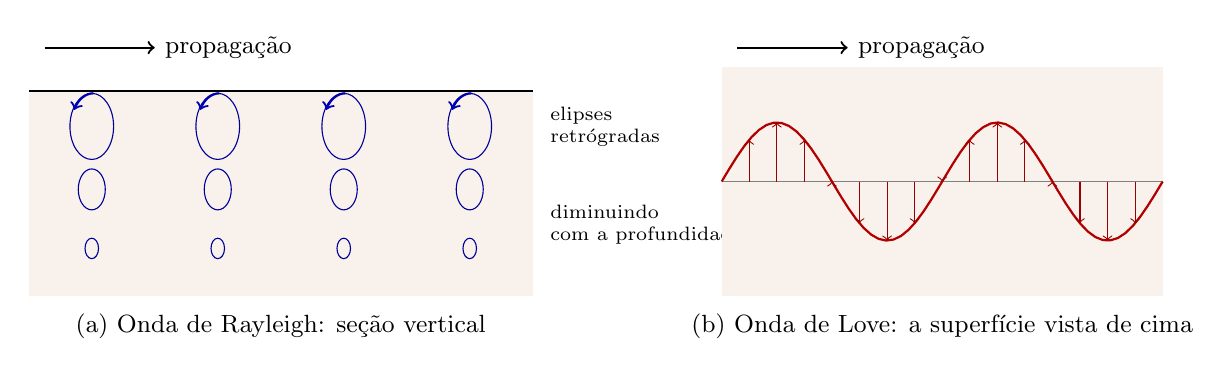
\begin{tikzpicture}[font=\small, x=1cm, y=1cm]
% Rayleigh: vertical section
\fill[brown!10] (0,0) rectangle (6.4,-2.6);
\draw[thick] (0,0) -- (6.4,0);
\draw[->, thick] (0.2,0.55) -- (1.6,0.55) node[right] {propagação};
\foreach \x/\s in {0.8/1, 2.4/-1, 4.0/1, 5.6/-1} {
  \foreach \z/\a in {-0.45/0.42, -1.25/0.26, -2.0/0.13} {
    \draw[blue!60!black] (\x,\z) ellipse ({0.66*\a} and {\a});
  }
}
\foreach \x in {0.8, 2.4, 4.0, 5.6} {
  \draw[->, blue!70!black, thick] (\x+0.02,-0.03) arc (90:150:{0.28} and {0.42});
}
\node[anchor=north] at (3.2,-2.7) {(a) Onda de Rayleigh: seção vertical};
\node[anchor=west, font=\scriptsize, align=left] at (6.5,-0.45) {elipses\\retrógradas};
\node[anchor=west, font=\scriptsize, align=left] at (6.5,-1.7) {diminuindo\\com a profundidade};
% Love: plan view of the surface
\begin{scope}[xshift=8.8cm]
\fill[brown!10] (0,0.3) rectangle (5.6,-2.6);
\draw[->, thick] (0.2,0.55) -- (1.6,0.55) node[right] {propagação};
\draw[gray, thin] (0,-1.15) -- (5.6,-1.15);
\draw[red!70!black, thick, domain=0:5.6, samples=60] plot (\x,{-1.15+0.75*sin(\x*360/2.8)});
\foreach \x in {0.35,0.7,...,5.3} {
  \pgfmathsetmacro{\d}{0.75*sin(\x*360/2.8)}
  \draw[->, red!60!black] (\x,-1.15) -- (\x,{-1.15+\d});
}
\node[anchor=north] at (2.8,-2.7) {(b) Onda de Love: a superfície vista de cima};
\end{scope}
\end{tikzpicture}

\par\smallskip{\small Movimentos das partículas das duas ondas de superfície (esquemático).
(a) Uma \omterm{def:b3:seismology-imaging:surface-waves}{onda de Rayleigh} move o solo no plano vertical de propagação,
ao longo de elipses que se invertem no topo (retrógradas) próximo à superfície e
diminuem com a profundidade. (b) Uma \omterm{def:b3:seismology-imaging:surface-waves}{onda de Love} move o solo horizontalmente, transversalmente à
direção de propagação: as setas mostram o deslocamento, em um instante,
ao longo de uma linha da superfície.}
\label{fig:b3:seismology-imaging:particle-motion}
\end{omfigure}

\begin{theorem}[Dispersão de ondas de Love em uma camada sobre um semiespaço]\label{thm:b3:seismology-imaging:love}
Uma camada de espessura $H$, módulo de cisalhamento $\mu_1$ e velocidade S $\beta_1$ repousa sobre um
semiespaço de módulo de cisalhamento $\mu_2$ e velocidade S $\beta_2 > \beta_1$. Uma
\omterm{def:b3:seismology-imaging:surface-waves}{onda de Love} de frequência angular $\omega$ e número de onda $k$ se propaga com a
velocidade de fase $c = \omega/k$, $\beta_1 < c < \beta_2$, se e somente se
\[
  \tan\!\left(kH q_1\right) = \frac{\mu_2 q_2}{\mu_1 q_1},
  \qquad q_1 = \sqrt{\frac{c^2}{\beta_1^2} - 1},\quad
  q_2 = \sqrt{1 - \frac{c^2}{\beta_2^2}} .
\]
O modo fundamental é a raiz com $0 < kHq_1 < \pi/2$; os harmônicos superiores têm
$kHq_1$ em $(n\pi, n\pi + \pi/2)$.
\end{theorem}

\begin{proof}
Tome $x$ na direção da propagação, $y$ horizontal e transversal a ela e $z$ para baixo, a partir da
superfície livre, e procure um deslocamento
$u_y = f(z)\,e^{i(kx - \omega t)}$, sendo as demais componentes nulas. Cada camada
obedece à equação de onda $\partial^2 u_y/\partial t^2 = \beta^2\nabla^2 u_y$, logo
$f'' = -k^2\left(c^2/\beta^2 - 1\right) f$. Na camada, $c > \beta_1$, e
$f = A\cos(kq_1z) + B\sin(kq_1z)$. No semiespaço, $c < \beta_2$, e a
solução que permanece limitada em profundidade é $f = C\,e^{-kq_2(z - H)}$.
A tensão de cisalhamento sobre um plano horizontal é $\mu\,\partial u_y/\partial z$.
Na superfície livre ela se anula: $f'(0) = 0$, donde $B = 0$. Em $z = H$, o
deslocamento e a tensão são contínuos:
\[
  A\cos(kq_1H) = C, \qquad -\mu_1 A\,kq_1\sin(kq_1H) = -\mu_2\,kq_2\,C .
\]
Dividindo a segunda equação pela primeira obtém-se o resultado. Como o
lado direito é positivo, $kHq_1$ fica em um quarto de período em que a
tangente é positiva; o menor desses intervalos fornece o modo fundamental.
\end{proof}

Para um dado período, a equação é resolvida para $c$ por bissecção; a
velocidade de grupo segue de $U = \mathrm d\omega/\mathrm dk$. Em períodos curtos
($kH$ grande), a raiz fica perto de $c = \beta_1$: a onda vive na camada. Em
períodos longos ($kH \to 0$), é preciso que $kHq_1 \to 0$ com o lado direito
também pequeno, o que força $c \to \beta_2$: a onda alcança fundo no semiespaço e
se propaga à sua velocidade. Entre os dois extremos, a velocidade de fase cresce
continuamente com o período.

\begin{definition}[Dispersão de ondas de superfície]\label{def:b3:seismology-imaging:dispersion}
A \emph{dispersão de ondas de superfície}\index{dispersão de ondas de superfície} é a dependência
das velocidades de fase e de grupo de uma \omterm{def:b3:seismology-imaging:surface-waves}{onda de Rayleigh} ou de Love em relação ao seu período. Em
uma Terra estratificada ela surge porque uma onda de período maior alcança maior profundidade
(cerca de um terço de um comprimento de onda, no modo fundamental) e faz média com rochas mais
rápidas; as curvas de dispersão $c(T)$ e $U(T)$ medidas entre um terremoto
e uma estação, ou entre duas estações, são invertidas para a velocidade S em
função da profundidade.
\end{definition}

\begin{omfigure}
\begin{tikzpicture}
\begin{axis}[omrecord, xmode=log, width=0.82\linewidth, height=0.5\linewidth,
  xmin=3, xmax=150, ymin=3.3, ymax=4.6, log basis x=10,
  xtick={3,5,10,20,50,100,150}, xticklabels={3,5,10,20,50,100,150},
  xlabel={período $T$ (\unit{s})}, ylabel={velocidade (\unit{km.s^{-1}})},
  legend style={at={(0.03,0.62)}, anchor=west}, legend cell align=left]
\addplot[blue!70!black, thick] table[x=period, y=c] {figdata/out/bachelor-3-love_dispersion-curve.dat};
\addlegendentry{velocidade de fase $c$}
\addplot[red!70!black, thick] table[x=period, y=U] {figdata/out/bachelor-3-love_dispersion-curve.dat};
\addlegendentry{velocidade de grupo $U$}
\draw[gray, dashed] (axis cs:3,3.5) -- (axis cs:150,3.5);
\draw[gray, dashed] (axis cs:3,4.5) -- (axis cs:150,4.5);
\node[font=\scriptsize, anchor=south] at (axis cs:80,3.5) {$\beta_1 = 3.5$};
\node[font=\scriptsize, anchor=south west] at (axis cs:3.1,4.5) {$\beta_2 = 4.5$};
\addplot[only marks, mark=*, mark size=1.4pt, red!70!black] coordinates {(19.2,3.384)};
\node[font=\scriptsize, anchor=south, red!70!black] at (axis cs:19.2,3.39) {fase de Airy};
\end{axis}
\end{tikzpicture}

\par\smallskip{\small \omterm{def:b3:seismology-imaging:surface-waves}{Ondas de Love} de modo fundamental numa camada de \qty{35}{km}
($\beta_1 = \qty{3.5}{km.s^{-1}}$, \qty{2.7}{g.cm^{-3}}) sobre um semiespaço
($\beta_2 = \qty{4.5}{km.s^{-1}}$, \qty{3.3}{g.cm^{-3}}), um modelo simplificado de uma
crosta continental sobre o manto, calculadas a partir
do \cref{thm:b3:seismology-imaging:love}. A velocidade de fase cresce desde a
velocidade S da camada até a do semiespaço; a velocidade de grupo é menor e tem um
mínimo, \qty{3.384}{km.s^{-1}} em \qty{19.2}{s}, onde ondas de períodos vizinhos
chegam juntas como um pulso tardio e amplo (a fase de Airy).}
\label{fig:b3:seismology-imaging:love}
\end{omfigure}

Neste modelo, a velocidade de fase em \qty{20}{s} é \qty{3.79}{km.s^{-1}} e em
\qty{100}{s} é \qty{4.444}{km.s^{-1}}; as velocidades de grupo são 3.384 e
\qty{4.333}{km.s^{-1}}. Num sismograma registrado a alguns milhares de quilômetros
de distância, os períodos longos chegam primeiro e as ondas de 20 s por último, de modo que o
trem de ondas se estende numa oscilação longa que lentamente se encurta. Medindo
a velocidade de grupo em muitos períodos, ao longo de muitos caminhos, fornece mapas
da espessura da crosta e da parte mais superior do manto, independentes dos
tempos de percurso das ondas de corpo.

\section{A Terra vibra: modos normais}

Uma onda de superfície de período muito longo tem um comprimento de onda comparável ao
raio da Terra; ela dá a volta no globo e encontra a si mesma. As ondas que
interferem construtivamente são as ondas estacionárias de toda a esfera, seus modos normais,
e, após um grande terremoto, são o último sinal a se extinguir.
Sua teoria, um problema de autovalores para a Terra elástica e autogravitante, está
além deste capítulo; sua descrição, porém, não.

Os modos de uma Terra com simetria esférica formam duas famílias. Nos
modos \emph{toroidais}, ${}_nT_\ell$, o movimento é horizontal, uma torção de
camadas esféricas umas contra as outras, sem variação de raio ou de volume: são as
ondas estacionárias das \omterm{def:b3:seismology-imaging:surface-waves}{ondas de Love}. Nos modos \emph{esferoidais}, ${}_nS_\ell$,
o movimento tem componentes radial e horizontal, e a Terra muda de forma: são as
ondas estacionárias das \omterm{def:b3:seismology-imaging:surface-waves}{ondas de Rayleigh}, acopladas às ondas de corpo e à gravidade.
O índice $\ell$ é o grau angular, o número de linhas nodais do
padrão na superfície; $n$ conta os nós do movimento com o raio, $n = 0$
para o modo fundamental. O modo esferoidal mais grave, ${}_0S_2$, estica a
Terra, alternadamente, em um esferoide prolato e em um oblato; o modo toroidal mais grave,
${}_0T_2$, torce os hemisférios norte e sul em
sentidos opostos. Seus períodos observados são:
\begin{center}
\small
% ledger: seis5:modes-T, seis5:modes-S
\begin{tabular}{lcccc}
\hline
modo & ${}_0T_2$ & ${}_1T_2$ & ${}_0T_3$ & ${}_1T_3$ \\
período (\unit{min}) & 44.01 & 12.61 & 28.43 & 11.59 \\
\hline
modo & ${}_0S_2$ & ${}_1S_2$ & ${}_0S_3$ & ${}_1S_3$ \\
período (\unit{min}) & 53.89 & 24.51 & 35.56 & 17.68 \\
\hline
\end{tabular}
\end{center}
Cada período é uma média sobre todo o planeta de seus módulos elásticos e
densidade, ponderada pelo local onde o modo se move: os modos toroidais sentem apenas o
manto sólido e a crosta, e os modos esferoidais também o núcleo. Ajustar os
períodos de centenas de modos é a única maneira sismológica de pesar o
interior: isso restringe a densidade, não apenas as velocidades, e o PREM foi construído para
ajustá-los em conjunto aos tempos de percurso. A rotação e a elipticidade da
Terra dividem cada modo de grau $\ell$ em $2\ell + 1$ frequências ligeiramente
diferentes, análogo ao efeito Zeeman.

\begin{history}[A Terra depois do terremoto chileno]
O terremoto chileno de 1960 foi registrado por sismômetros pendulares de longo período
e por extensômetros, instrumentos que medem a variação de comprimento de uma
haste ou fio horizontal longo ancorado na rocha. A análise espectral de alguns dias de
registro mostrou picos nítidos nos períodos previstos dos modos mais graves: a
Terra inteira havia entrado em vibração, e as previsões da teoria elástica
de uma Terra esférica e autogravitante se confirmaram. O registro do extensômetro
em Isabella, na Califórnia, foi analisado novamente em 1978 com métodos mais modernos:
ele mostrou claramente o desdobramento de ${}_0T_3$, ${}_0T_4$, ${}_0S_4$
e ${}_0S_5$ pela rotação e pela elipticidade da Terra, e confirmou também o
desdobramento de ${}_0S_2$ e ${}_0S_3$.
% ledger: stein78:chile-modes, usgs5:chile1960
A sismologia de modos normais, nascida de um único terremoto, hoje usa as redes de
estações de banda muito larga que registram todo grande terremoto.
\end{history}

\section{Problemas inversos lineares}\label{sec:b3:seismology-imaging:inverse}

Todos os métodos deste capítulo até aqui calculam dados a partir de um modelo. A tarefa do
imageamento é o inverso.

\begin{definition}[Problema direto, problema inverso]\label{def:b3:seismology-imaging:inverse}
Suponha-se que um modelo da Terra seja descrito por um vetor $\mathbf m$ de $M$ parâmetros
e as observações por um vetor $\mathbf d$ de $N$ dados. O \emph{problema
direto}\index{problema direto} consiste em calcular os dados $\mathbf d = g(\mathbf m)$
que um dado modelo produziria, segundo uma teoria física. O \emph{problema
inverso}\index{problema inverso} consiste em estimar o modelo a partir de dados que
trazem erros, $\mathbf d = g(\mathbf m) + \mathbf e$, e em dizer quão bem cada parte
do modelo está determinada. O problema é linear quando $g(\mathbf m) =
\mathsf G\mathbf m$ para uma matriz fixa $N\times M$ $\mathsf G$, o núcleo.
\end{definition}

Ajustar uma reta a tempos de percurso é um \omterm{def:b3:seismology-imaging:inverse}{problema inverso} linear com
$M = 2$ (exercício 7); uma tomografia de tempos de percurso tem milhares de
parâmetros. Surgem três casos. Se $N > M$ e os dados restringem todos os
parâmetros, o problema é \emph{sobredeterminado}: nenhum modelo ajusta cada dado
exatamente, e busca-se o melhor no sentido estatístico. Se alguma combinação dos
parâmetros deixa os dados inalterados ($\mathsf G\mathbf m_0 = \mathbf 0$ para
algum $\mathbf m_0 \ne \mathbf 0$), o problema é \emph{subdeterminado} nessa
direção, e nenhuma quantidade de dados desse tipo a fixará. Problemas reais são
mistos: sobredeterminados em algumas partes do modelo e subdeterminados em
outras.

\begin{theorem}[Estimativa de mínimos quadrados ponderados]\label{thm:b3:seismology-imaging:wls}
Seja $\mathbf d = \mathsf G\mathbf m + \mathbf e$, em que os erros $\mathbf e$
têm média zero e a matriz de covariância $\mathsf C_d$ (diagonal
$\sigma_i^2$ para erros independentes). Se a matriz
$\mathsf N = \mathsf G^{\mathsf T}\mathsf C_d^{-1}\mathsf G$ é inversível, o
modelo que minimiza o desajuste
\[
  \chi^2(\mathbf m) = (\mathbf d - \mathsf G\mathbf m)^{\mathsf T}\mathsf C_d^{-1}
  (\mathbf d - \mathsf G\mathbf m)
\]
é a \emph{estimativa de mínimos quadrados ponderados}\index{estimativa de mínimos quadrados ponderados}
\[
  \hat{\mathbf m} = \mathsf N^{-1}\mathsf G^{\mathsf T}\mathsf C_d^{-1}\mathbf d ,
\]
ele é não enviesado, e sua matriz de covariância é
$\mathsf C_{\hat m} = \mathsf N^{-1}$.
\end{theorem}

\begin{proof}
$\chi^2$ é uma função quadrática de $\mathbf m$ com gradiente
$-2\mathsf G^{\mathsf T}\mathsf C_d^{-1}(\mathbf d - \mathsf G\mathbf m)$, que
se anula para as equações normais $\mathsf N\mathbf m = \mathsf G^{\mathsf T}
\mathsf C_d^{-1}\mathbf d$; a hessiana $2\mathsf N$ é definida positiva quando
$\mathsf N$ é invertível (então $\mathbf x^{\mathsf T}\mathsf N\mathbf x =
\|\mathsf C_d^{-1/2}\mathsf G\mathbf x\|^2 > 0$ para $\mathbf x \ne 0$), de modo que o
ponto estacionário é o mínimo. Escreve-se $\hat{\mathbf m} = \mathsf H\mathbf d$ com
$\mathsf H = \mathsf N^{-1}\mathsf G^{\mathsf T}\mathsf C_d^{-1}$. Então
$\mathsf H\mathsf G = \mathsf I$, de modo que $\hat{\mathbf m} = \mathbf m + \mathsf H\mathbf e$
tem média $\mathbf m$, e sua covariância é
$\mathsf H\mathsf C_d\mathsf H^{\mathsf T} =
\mathsf N^{-1}\mathsf G^{\mathsf T}\mathsf C_d^{-1}\mathsf C_d\mathsf C_d^{-1}
\mathsf G\mathsf N^{-1} = \mathsf N^{-1}$.
\end{proof}

Os pesos fazem o que a intuição pede: um dado com metade do erro conta
quatro vezes mais. A matriz de covariância fornece a cada parâmetro seu erro padrão
$\sqrt{(\mathsf N^{-1})_{jj}}$ e as correlações entre eles. Se o modelo
estiver correto e os erros forem gaussianos, o mínimo $\chi^2$ segue uma lei $\chi^2$
com $N - M$ graus de liberdade: um valor muito acima de $N - M$ indica que os erros
foram subestimados ou que o modelo é simples demais; muito abaixo, que os erros
foram superestimados.

Quando $\mathsf N$ é singular ou quase singular, a estimativa não existe ou é
dominada por ruído amplificado nas direções mal restringidas. O remédio
padrão é buscar um modelo que ajuste os dados razoavelmente e não seja
desnecessariamente grande.

\begin{definition}[Mínimos quadrados amortecidos, curva de compromisso]\label{def:b3:seismology-imaging:damped}
Para um parâmetro de amortecimento $\varepsilon > 0$, a estimativa por \emph{mínimos quadrados amortecidos}\index{mínimos quadrados amortecidos}
é o modelo que minimiza
\[
  \Phi_\varepsilon(\mathbf m) = \chi^2(\mathbf m) + \varepsilon^2\|\mathbf m\|^2 ,
  \qquad
  \mathbf m_\varepsilon = \left(\mathsf N + \varepsilon^2\mathsf I\right)^{-1}
  \mathsf G^{\mathsf T}\mathsf C_d^{-1}\mathbf d .
\]
A \emph{curva de compromisso}\index{curva de compromisso} é a curva traçada, à medida que
$\varepsilon$ varia, pelo par (tamanho do modelo $\|\mathbf m_\varepsilon\|$,
desajuste $\chi^2(\mathbf m_\varepsilon)$): amortecimento pequeno ajusta os dados de perto
com um modelo grande e irregular; amortecimento grande fornece um modelo pequeno e um ajuste ruim.
\end{definition}

A fórmula se obtém como no \cref{thm:b3:seismology-imaging:wls}: o gradiente
de $\Phi_\varepsilon$ é $-2\mathsf G^{\mathsf T}\mathsf C_d^{-1}(\mathbf d -
\mathsf G\mathbf m) + 2\varepsilon^2\mathbf m$, e $\mathsf N + \varepsilon^2
\mathsf I$ é sempre invertível, pois seus autovalores são os de
$\mathsf N$ (todos $\ge 0$) acrescidos de $\varepsilon^2$. O amortecimento costuma ser
escolhido perto do joelho da \omterm{def:b3:seismology-imaging:damped}{curva de compromisso}, ou de modo que $\chi^2$ seja aproximadamente
o número de dados, o desajuste esperado apenas pelos erros. O preço é que a
estimativa deixa de ser não enviesada.

\begin{definition}[Matriz de resolução do modelo]\label{def:b3:seismology-imaging:resolution}
Para uma estimativa linear $\mathbf m_\varepsilon = \mathsf H_\varepsilon \mathbf d$
do modelo $\mathbf m$ a partir dos dados $\mathbf d = \mathsf G\mathbf m + \mathbf e$,
a \emph{matriz de resolução do modelo}\index{matriz de resolução do modelo} é
$\mathsf R = \mathsf H_\varepsilon\mathsf G$, de modo que
\[
  \mathbf m_\varepsilon = \mathsf R\,\mathbf m + \mathsf H_\varepsilon\mathbf e .
\]
Para \omterm{def:b3:seismology-imaging:damped}{mínimos quadrados amortecidos}, $\mathsf R = (\mathsf N + \varepsilon^2\mathsf I)^{-1}
\mathsf N$. A linha $j$ de $\mathsf R$ mostra como a estimativa do parâmetro $j$
faz média dos parâmetros verdadeiros; $\mathsf R = \mathsf I$ significa resolução perfeita.
\end{definition}

Se $\mathsf N$ tem os autovetores ortonormais $\mathbf u_k$ e os autovalores
$\lambda_k$, então $\mathsf R = \sum_k \frac{\lambda_k}{\lambda_k + \varepsilon^2}
\mathbf u_k\mathbf u_k^{\mathsf T}$: as direções que os dados restringem bem
($\lambda_k \gg \varepsilon^2$) passam quase inalteradas, enquanto aquelas que restringem
mal são suprimidas. O traço de $\mathsf R$ conta os parâmetros que os dados
efetivamente resolvem, e a covariância da estimativa,
$\mathsf H_\varepsilon\mathsf C_d\mathsf H_\varepsilon^{\mathsf T}$, diminui à medida que
a resolução diminui: o amortecimento troca resolução por estabilidade.

\begin{omfigure}
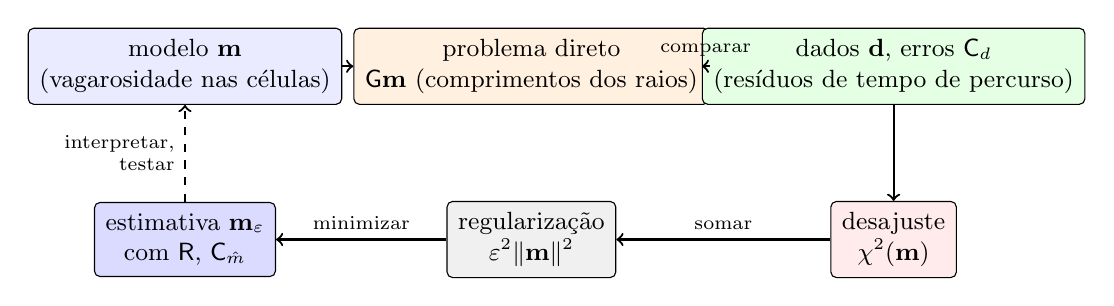
\begin{tikzpicture}[font=\small, node distance=0.5cm,
  box/.style={draw, rounded corners=2pt, fill=#1, minimum height=0.9cm, align=center, inner sep=4pt},
  box/.default=gray!8]
\node[box=blue!8] (m) at (0,0) {modelo $\mathbf m$\\(vagarosidade nas células)};
\node[box=orange!12] (g) at (4.4,0) {problema direto\\$\mathsf G\mathbf m$ (comprimentos dos raios)};
\node[box=green!10] (d) at (9.0,0) {dados $\mathbf d$, erros $\mathsf C_d$\\(resíduos de tempo de percurso)};
\node[box=red!8] (mis) at (9.0,-2.2) {desajuste\\$\chi^2(\mathbf m)$};
\node[box=gray!12] (reg) at (4.4,-2.2) {regularização\\$\varepsilon^2\|\mathbf m\|^2$};
\node[box=blue!14] (est) at (0,-2.2) {estimativa $\mathbf m_\varepsilon$\\com $\mathsf R$, $\mathsf C_{\hat m}$};
\draw[->, thick] (m) -- (g);
\draw[->, thick] (g) -- node[above, font=\scriptsize] {comparar} (d);
\draw[->, thick] (d) -- (mis);
\draw[->, thick] (mis) -- node[above, font=\scriptsize] {somar} (reg);
\draw[->, thick] (reg) -- node[above, font=\scriptsize] {minimizar} (est);
\draw[->, thick, dashed] (est) -- node[left, font=\scriptsize, align=right] {interpretar,\\testar} (m);
\end{tikzpicture}

\par\smallskip{\small O \omterm{def:b3:seismology-imaging:inverse}{problema inverso} linear como um ciclo (esquemático). O
\omterm{def:b3:seismology-imaging:inverse}{problema direto} prevê dados a partir de um modelo; o desajuste, ponderado pelos
erros dos dados, mede a discordância; o termo de regularização mantém o modelo
pequeno; minimizar a soma dos dois fornece a estimativa, que só é interpretável
junto com sua matriz de resolução e sua covariância.}
\label{fig:b3:seismology-imaging:inverse-loop}
\end{omfigure}

\section{Tomografia sísmica}\label{sec:b3:seismology-imaging:tomography}

\begin{definition}[Tomografia sísmica, resíduo de tempo de percurso]\label{def:b3:seismology-imaging:tomography}
O \emph{resíduo de tempo de percurso}\index{resíduo de tempo de percurso} de uma chegada é o
tempo de percurso observado menos o tempo previsto por um modelo de referência,
$\delta t = T_{\text{obs}} - T_{\text{ref}}$, após a correção para a localização da fonte
e o tempo de origem, a elevação da estação e a elipticidade da Terra.
A \emph{tomografia sísmica}\index{tomografia sísmica} é a
estimativa dos desvios tridimensionais das velocidades sísmicas em relação a um
modelo de referência, $\delta v(\mathbf x)$, a partir de um grande conjunto de resíduos (ou de
formas de onda), por meio da resolução de um \omterm{def:b3:seismology-imaging:inverse}{problema inverso}.
\end{definition}

Denota-se $s = 1/v$ a vagarosidade. O tempo de percurso ao longo de um raio $\Gamma$ é
$T = \int_\Gamma s\,\mathrm dl$; porém o próprio raio depende das velocidades,
o que parece tornar o problema não linear. A resposta de primeira ordem é que isso
não importa.

\begin{proposition}[Resíduo de tempo de percurso linearizado]\label{prop:b3:seismology-imaging:linear}
Se a vagarosidade do modelo de referência $s_0$ for perturbada para $s_0 + \delta s$,
o tempo de percurso entre dois pontos fixos varia, em primeira ordem em
$\delta s$, por
\[
  \delta t = \int_{\Gamma_0}\delta s\,\mathrm dl ,
\]
a integral sendo tomada ao longo do raio $\Gamma_0$ do modelo de referência; a
anomalia relativa de velocidade é $\delta v/v_0 = -\delta s/s_0$, na mesma ordem.
\end{proposition}

\begin{proof}
Pelo princípio de Fermat, o raio $\Gamma_0$ torna o tempo de percurso
$\int s_0\,\mathrm dl$ estacionário entre caminhos vizinhos: deslocando o caminho por uma
pequena quantidade $\epsilon$, o tempo varia apenas por um termo de ordem $\epsilon^2$.
O novo raio $\Gamma$ difere de $\Gamma_0$ por uma quantidade de ordem $\delta s$;
logo $\int_\Gamma(s_0 + \delta s)\,\mathrm dl = \int_{\Gamma_0}s_0\,\mathrm dl +
O(\delta s^2) + \int_{\Gamma_0}\delta s\,\mathrm dl + O(\delta s^2)$. Por fim
$\delta(1/s) = -\delta s/s_0^2$, logo $\delta v/v_0 = -\delta s/s_0$.
\end{proof}

Divide-se a região em $M$ células de perturbação uniforme da vagarosidade $\delta s_j$.
O resíduo do raio $i$ torna-se $\delta t_i = \sum_j L_{ij}\,\delta s_j$, em que
$L_{ij}$ é o comprimento do raio de referência $i$ na célula $j$: um \omterm{def:b3:seismology-imaging:inverse}{problema inverso} linear
cujo núcleo é a matriz de comprimentos dos raios, cujas entradas são quase todas
nulas. Os resíduos são pequenos: em um manto a
\qty{8}{km.s^{-1}}, uma região de \qty{200}{km} de largura que é \qty{3}{\percent}
mais rápida adianta um raio vertical em cerca de \qty{0.7}{s} (exercício 9).

\begin{method}[Tomografia por tempos de percurso]\label{met:b3:seismology-imaging:tomo}
\begin{enumerate}
  \item Selecionam-se os tempos de chegada de uma fase (por exemplo, P) em todas as estações, para
        terremotos cuja localização seja bem conhecida; calculam-se os resíduos
        em relação a uma \omterm{def:b3:seismology-imaging:tables}{tabela de tempos de percurso}, corrigidos para a elipticidade e a elevação da
        estação.
  \item Traçam-se os raios de referência e divide-se a região em células (ou expande-se
        $\delta s$ em funções suaves); preenche-se a matriz de comprimentos dos raios.
  \item Atribui-se a cada resíduo seu erro, a partir da precisão da leitura, e resolve-se
        o problema de \omterm{def:b3:seismology-imaging:damped}{mínimos quadrados amortecidos} para uma faixa de valores de amortecimento; traça-se
        a \omterm{def:b3:seismology-imaging:damped}{curva de compromisso} e escolhe-se o amortecimento próximo de seu joelho.
  \item Testa-se a resolução: calculam-se os resíduos que um modelo sintético conhecido
        produziria pelos mesmos raios, acrescenta-se ruído, inverte-se com o
        mesmo amortecimento, e compara-se.
  \item Interpretam-se apenas as anomalias que o teste mostra que os raios podem
        recuperar, com suas amplitudes entendidas como limites inferiores.
\end{enumerate}
\end{method}

\begin{definition}[Teste do tabuleiro de xadrez]\label{def:b3:seismology-imaging:checkerboard}
Um \emph{teste do tabuleiro de xadrez}\index{teste do tabuleiro de xadrez} é um teste de resolução em
no qual o modelo sintético é um padrão regular de células alternadamente rápidas e lentas:
resíduos sintéticos calculados pela geometria real dos raios, com ruído
de mesma magnitude dos erros reais, são invertidos com a mesma parametrização e
amortecimento. Onde o padrão é recuperado, estruturas desse tamanho podem ser
resolvidas; onde ele é borrado ou perdido, não podem.
\end{definition}

As figuras abaixo realizam o teste em uma seção de modelo com \qty{800}{km} de largura e
\qty{400}{km} de profundidade, dividida em 128 células de \qty{50}{km}. Vinte fontes situam-se
ao longo de sua base e trinta e duas estações ao longo de seu topo, e somente os raios dentro
de \ang{45} da vertical são usados: 480 raios que percorrem, todos, de forma íngreme, o caminho para cima,
a geometria de raios de terremotos distantes subindo sob uma rede.
O modelo sintético tem blocos de $2\times2$ células, com \qty{3}{\percent} mais rápidos ou mais lentos
em torno de \qty{8}{km.s^{-1}}; os resíduos carregam ruído gaussiano de
\qty{0.05}{s}.
% figdata: tomo_checkerboard.py (invented geometry; no real data)

\begin{omfigure}
\begin{tikzpicture}
\begin{groupplot}[group style={group size=2 by 2, horizontal sep=0.9cm, vertical sep=1.25cm},
  width=0.46\linewidth, height=0.3\linewidth, xmin=0, xmax=800, ymin=0, ymax=400,
  axis on top, enlargelimits=false, tick label style={font=\scriptsize},
  title style={font=\small, yshift=-1ex},
  colormap={tomo}{rgb255(0cm)=(178,24,43); rgb255(1cm)=(244,165,130); rgb255(2cm)=(247,247,247); rgb255(3cm)=(146,197,222); rgb255(4cm)=(33,102,172)},
  point meta min=-4, point meta max=4]
\nextgroupplot[title={(a) modelo sintético}, ylabel={\scriptsize altura (km)}]
\addplot[matrix plot*, mesh/cols=16, point meta=explicit] table[x=x, y=y, meta=dv] {figdata/out/bachelor-3-tomo_checkerboard-true.dat};
\nextgroupplot[title={(b) uma amostra dos 480 raios}, colormap/blackwhite]
\addplot[gray!70!black, thin, unbounded coords=jump] table[x=x, y=y] {figdata/out/bachelor-3-tomo_checkerboard-rays.dat};
\addplot[only marks, mark=triangle*, mark size=1.6pt, black, clip=false] table[x=x, y=y] {figdata/out/bachelor-3-tomo_checkerboard-receivers.dat};
\addplot[only marks, mark=star, mark size=1.8pt, red!70!black, clip=false] table[x=x, y=y] {figdata/out/bachelor-3-tomo_checkerboard-sources.dat};
\nextgroupplot[title={(c) recuperado, $\varepsilon = \qty{3}{km}$}, ylabel={\scriptsize altura (km)}, xlabel={\scriptsize distância (km)}]
\addplot[matrix plot*, mesh/cols=16, point meta=explicit] table[x=x, y=y, meta=dv] {figdata/out/bachelor-3-tomo_checkerboard-rec-low.dat};
\nextgroupplot[title={(d) recuperado, $\varepsilon = \qty{60}{km}$}, xlabel={\scriptsize distância (km)},
  colorbar right, colorbar style={width=0.2cm, ytick={-4,-2,0,2,4}, ylabel={\scriptsize $\delta v/v$ (\%)}, tick label style={font=\scriptsize}}]
\addplot[matrix plot*, mesh/cols=16, point meta=explicit] table[x=x, y=y, meta=dv] {figdata/out/bachelor-3-tomo_checkerboard-rec-high.dat};
\end{groupplot}
\end{tikzpicture}

\par\smallskip{\small Um \omterm{def:b3:seismology-imaging:checkerboard}{teste do tabuleiro de xadrez} (geometria inventada). (a) O
modelo sintético: blocos de \qty{100}{km} de largura, \qty{3}{\percent} mais rápidos (azul) ou
mais lentos (vermelho). (b) As 20 fontes (estrelas), as 32
estações (triângulos) e alguns dos raios, todos dentro de \ang{45} da vertical. (c) Com
amortecimento leve os blocos são recuperados, porém ruidosos, com anomalias de até cerca de
\qty{8}{\percent} onde poucos raios se cruzam (as cores saturam em
\qty{4}{\percent}). (d) Com amortecimento forte o padrão fica limpo, porém sua
amplitude é reduzida, sobretudo ao longo das bordas laterais, onde poucos raios se cruzam
e todos em ângulos semelhantes.}
\label{fig:b3:seismology-imaging:checkerboard}
\end{omfigure}

\begin{omfigure}
\begin{tikzpicture}
\begin{axis}[omrecord, width=0.62\linewidth, height=0.42\linewidth,
  xlabel={norma do modelo $\|\delta v/v\|$ (\unit{\percent})},
  ylabel={desajuste $\|\mathsf G\mathbf m - \mathbf d\|$ (\unit{s})}, xmin=0, xmax=42, ymin=0, ymax=12]
\addplot[blue!70!black, thick] table[x=norm, y=misfit] {figdata/out/bachelor-3-tomo_checkerboard-tradeoff.dat};
\addplot[only marks, mark=*, mark size=1.8pt, red!70!black] coordinates {(38.84,0.862) (29.42,1.159)};
\node[font=\scriptsize, anchor=south, red!70!black] at (axis cs:38.84,1.3) {$\varepsilon = 3$};
\node[font=\scriptsize, anchor=east, red!70!black] at (axis cs:28.6,0.55) {$\varepsilon = 60$};
\draw[gray, dashed] (axis cs:0,1.095) -- (axis cs:42,1.095);
\node[font=\scriptsize, anchor=south west] at (axis cs:1,1.15) {esperado a partir do ruído};
\draw[green!45!black, densely dotted] (axis cs:33.94,0) -- (axis cs:33.94,12);
\node[font=\scriptsize, anchor=north west, green!45!black] at (axis cs:34.2,11.8) {modelo verdadeiro};
\node[font=\scriptsize, anchor=west] at (axis cs:14,10.5) {amortecimento forte};
\node[font=\scriptsize, anchor=east] at (axis cs:41,3.2) {amortecimento leve};
\end{axis}
\end{tikzpicture}

\par\smallskip{\small A \omterm{def:b3:seismology-imaging:damped}{curva de compromisso} do \omterm{def:b3:seismology-imaging:checkerboard}{teste do tabuleiro de xadrez}, para o amortecimento
valores $\varepsilon$ de 0.1 a \qty{1000}{km} (o núcleo está em quilômetros,
com erros iguais). Ao longo do trecho plano, mais amortecimento custa quase nenhum ajuste: o
modelo encolhe ao perder ruído. O joelho situa-se onde o desajuste ultrapassa o
nível esperado apenas do ruído, $\sigma\sqrt{480} = \qty{1.095}{s}$; os
dois modelos amortecidos da figura anterior situam-se um de cada lado dele, e a
norma do tabuleiro de xadrez verdadeiro, \qty{33.9}{\percent}, fica entre eles. Além do
joelho, o amortecimento remove estrutura que os dados exigem.}
\label{fig:b3:seismology-imaging:tradeoff}
\end{omfigure}

O teste ilustra os três limites de toda imagem tomográfica. A resolução
é definida pelos raios: onde todos os raios são paralelos, uma anomalia fica espalhada ao longo
deles, e uma célula atravessada por poucos raios é mal restringida. O amortecimento reduz as
amplitudes: as anomalias recuperadas são limites inferiores.
E a imagem depende do modelo de referência e da parametrização: apenas os
desvios em relação à referência são mapeados, e nada menor que uma célula.
Com essas ressalvas, as imagens globais das ondas P e S mostram as lajes do
volume do primeiro ano (em seu capítulo sobre subducção) como regiões rápidas e tabulares que descem
das fossas oceânicas, algumas achatando-se acima da descontinuidade dos 670 km, outras
mergulhando no manto inferior; e amplas regiões lentas sob o Pacífico e
a África, sobre o núcleo, com condutos lentos mais estreitos sob alguns pontos quentes, candidatos
às plumas do manto do mesmo volume.

\begin{inthefield}[Uma estação de banda larga e uma implantação no fundo oceânico]
\begin{minipage}[t]{0.55\linewidth}\vspace{0pt}
Uma estação permanente de banda larga é um lugar silencioso: o sismômetro fica sobre um
pilar de concreto fixado ao embasamento rochoso, em um cofre enterrado ou em um túnel curto, sob um
escudo térmico, porque uma corrente de ar ou uma variação de algumas centésimas de grau
inclina o instrumento mais do que um terremoto distante. Suas três componentes,
vertical, norte e leste, são digitalizadas continuamente e enviadas a um centro de dados
com carimbo de tempo por satélite. Para imagear uma região sob o oceano, uma equipe de levantamento
lança sismômetros de fundo oceânico a partir de um navio: cada um afunda com uma âncora,
registra por um ano no fundo do mar e volta à superfície quando o navio
retorna e envia um sinal acústico para liberá-lo. A tripulação então lê seu
desvio de relógio, corrige os registros e acrescenta milhares de chegadas à
tomografia.
\end{minipage}\hfill
\begin{minipage}[t]{0.42\linewidth}\vspace{0pt}
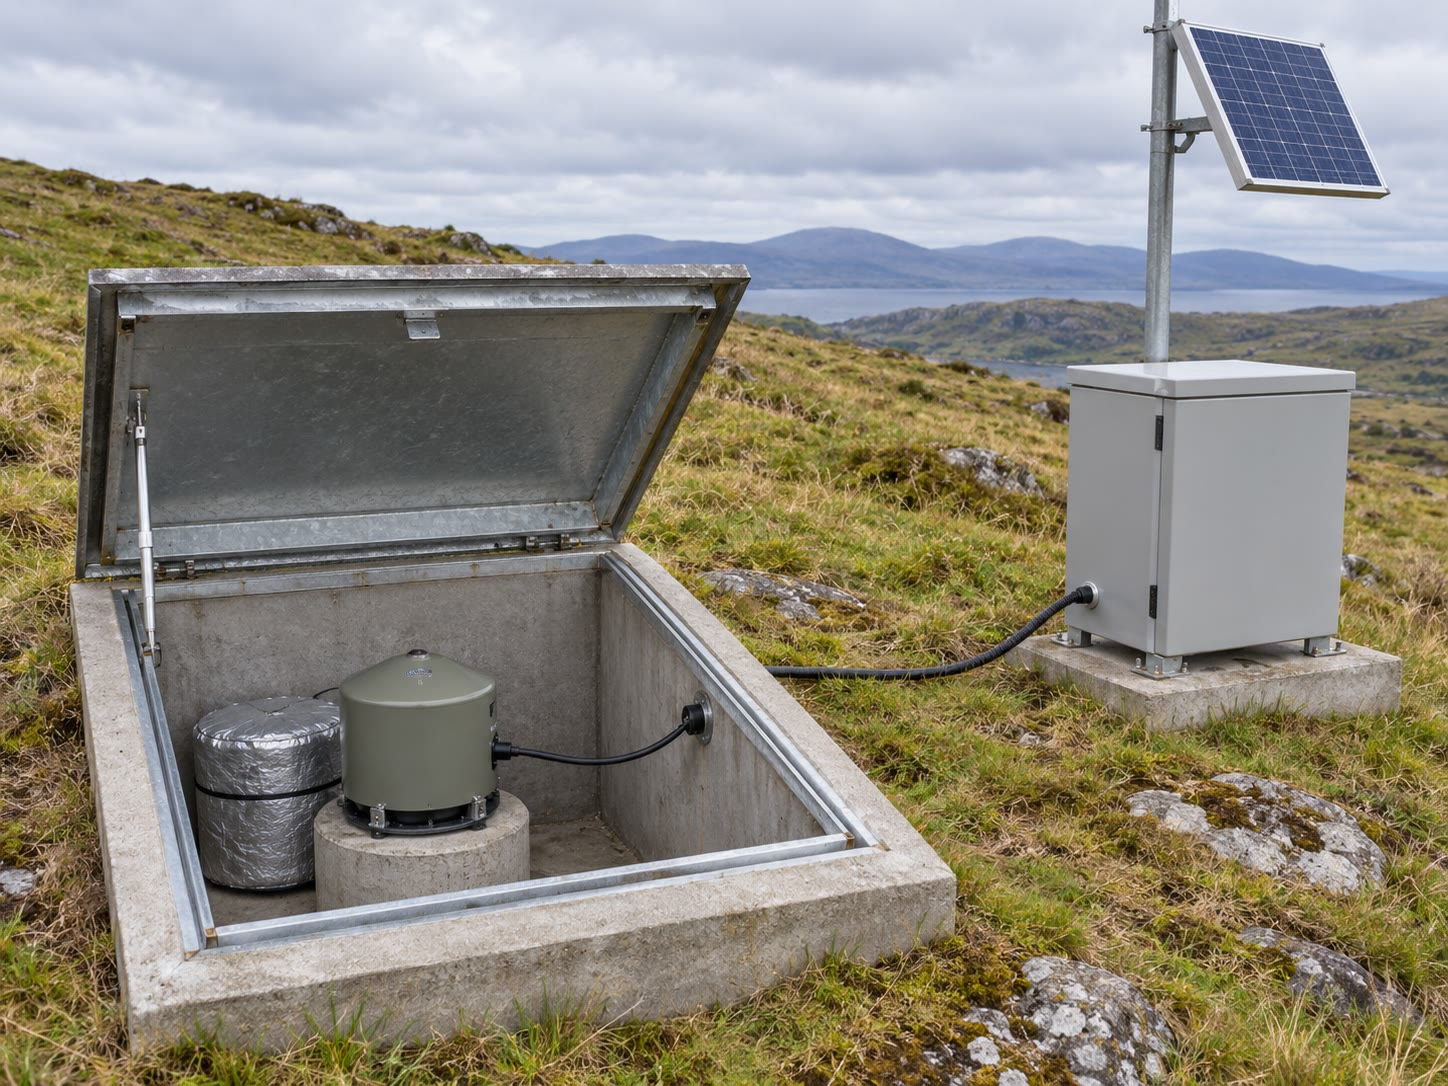
\includegraphics[width=\linewidth]{images/book5/ai/b3-seismic-vault.jpg}

{\scriptsize Um sismômetro de banda larga sobre seu pilar em um cofre de estação
Ilustração gerada por IA.}
\end{minipage}
\end{inthefield}

\section{Exercícios}

\begin{exercise}[$\star$]\label{exo:b3:seismology-imaging:1}
Um raio P deixa a superfície ($R = \qty{6371}{km}$, $v_0 = \qty{5.80}{km.s^{-1}}$)
com o \omterm{def:b3:seismology-imaging:ray-parameter}{parâmetro do raio} $p = \qty{500}{s.rad^{-1}}$. (a) Calcule seu ângulo de
emergência. (b) O PREM fornece velocidades P de \qty{11.066}{km.s^{-1}} na profundidade de \qty{771}{km}
e \qty{11.245}{km.s^{-1}} a \qty{871}{km}. Calcule $r/v$ nas duas profundidades e
determine a profundidade do ponto de retorno do raio por interpolação linear.
% ledger: ak135:crust, data:prem
\end{exercise}

\begin{exercise}[$\star$]\label{exo:b3:seismology-imaging:2}
Os tempos P calculados com o PREM neste capítulo são \qty{369.6}{s} a \ang{30}
e \qty{455.5}{s} a \ang{40}. (a) Estime a inclinação da curva de tempo de percurso
entre esses dois pontos, em \unit{s} por grau e em \unit{s.rad^{-1}}. (b) Deduza
a velocidade aparente da frente de onda ao longo da superfície, em
\unit{km.s^{-1}}. (c) Qual é a velocidade P no ponto de retorno do raio
que chega a \ang{35}, se ele retorna no raio \qty{5450}{km}?
\end{exercise}

\begin{exercise}[$\star$]\label{exo:b3:seismology-imaging:3}
No modelo de \omterm{def:b3:seismology-imaging:surface-waves}{onda de Love} deste capítulo, a camada tem $\beta_1 =
\qty{3.5}{km.s^{-1}}$, $\rho_1 = \qty{2700}{kg.m^{-3}}$ e o semiespaço
$\beta_2 = \qty{4.5}{km.s^{-1}}$, $\rho_2 = \qty{3300}{kg.m^{-3}}$.
(a) Calcule os dois módulos de cisalhamento. (b) Em \qty{20}{s}, a velocidade de fase é
\qty{3.79}{km.s^{-1}}: calcule o comprimento de onda e compare-o com a espessura da
camada, \qty{35}{km}. (c) Com velocidades de grupo de \qty{3.384}{km.s^{-1}} a
\qty{20}{s} e \qty{4.333}{km.s^{-1}} a \qty{100}{s}, em quantos minutos
as ondas de 20 s chegam depois das de 100 s numa estação a \qty{4000}{km} de distância?
\end{exercise}

\begin{exercise}[$\star$]\label{exo:b3:seismology-imaging:4}
Os períodos observados de ${}_0S_2$ e ${}_0T_2$ são \qty{53.89}{min} e
\qty{44.01}{min}. (a) Calcule suas frequências em \unit{mHz}. (b) Quantas
oscilações de cada um a Terra completa em um dia? (c) Dois picos espectrais
podem ser separados somente se o registro durar pelo menos o inverso de sua
diferença de frequência. Quanto deve durar um registro para separar esses dois modos?
% ledger: seis5:modes-S, seis5:modes-T
\end{exercise}

\begin{exercise}[$\star\star$]\label{exo:b3:seismology-imaging:5}
Em uma esfera de raio $R$ e velocidade uniforme $v$, os raios são cordas retas.
(a) Mostre que o raio que atinge $\Delta$ tem o tempo de percurso
$T = 2R\sin(\Delta/2)/v$. (b) Com $R = \qty{6371}{km}$ e
$v = \qty{10.0}{km.s^{-1}}$, calcule $T$ a \ang{30} e \ang{90}, e compare
com os tempos do PREM, \qty{369.6}{s} e \qty{779.7}{s}. (c) Explique por que a
esfera uniforme é rápida demais a \ang{30} e lenta demais a \ang{90}.
\end{exercise}

\begin{exercise}[$\star\star$]\label{exo:b3:seismology-imaging:6}
Em um sólido de Poisson ($\lambda = \mu$, logo $\alpha^2 = 3\beta^2$) a \omterm{def:b3:seismology-imaging:surface-waves}{onda de Rayleigh}
velocidade $c$ satisfaz, com $\xi = c^2/\beta^2$,
$(2 - \xi)^2 = 4\sqrt{1 - \xi/3}\,\sqrt{1 - \xi}$. (a) Eleve-a ao quadrado e mostre
que as raízes satisfazem $(\xi - 4)(3\xi^2 - 12\xi + 8) = 0$. (b) Mostre que a
única raiz com $0 < \xi < 1$ é $\xi = 2 - 2/\sqrt3$, e calcule $c/\beta$.
(c) Na crosta superior do ak135, $\beta = \qty{3.46}{km.s^{-1}}$: calcule a
velocidade de Rayleigh e o atraso da \omterm{def:b3:seismology-imaging:surface-waves}{onda de Rayleigh} em relação à onda S a
\qty{1000}{km}.
% ledger: ak135:crust
\end{exercise}

\begin{exercise}[$\star\star$]\label{exo:b3:seismology-imaging:7}
Chegadas de onda de cabeça em quatro estações de uma linha de refração, a 50, 100, 150 e
\qty{200}{km} do tiro, são 9.0, 15.3, 21.5 e \qty{27.9}{s}, com
erros de 0.1, 0.1, 0.2 e \qty{0.2}{s}. Ajuste $T = a + bx$ por mínimos quadrados
ponderados: escreva $\mathsf G$ e $\mathsf C_d$, forme as equações normais, e
dê $a$, $b$, seus erros padrão, a velocidade $1/b$ com seu erro, e o
mínimo $\chi^2$. O ajuste é aceitável?
\end{exercise}

\begin{exercise}[$\star\star$]\label{exo:b3:seismology-imaging:8}
Um raio atravessa duas células, com comprimentos \qty{30}{km} e \qty{40}{km}, e tem
um resíduo de \qty{0.50}{s}. (a) Por que $\mathsf N = \mathsf G^{\mathsf T}
\mathsf G$ é singular? (b) Entre os modelos que ajustam exatamente o resíduo, aquele
de menor norma é $\mathbf m = \mathsf G^{\mathsf T}(\mathsf G\mathsf
G^{\mathsf T})^{-1}\mathbf d$: calcule-o. (c) Calcule a matriz
$\mathsf R = \mathsf G^{\mathsf T}(\mathsf G\mathsf G^{\mathsf T})^{-1}\mathsf G$
e seu traço. (d) Se a anomalia verdadeira for \qty{0.01}{s.km^{-1}} apenas na primeira
célula, o que se recupera?
\end{exercise}

\begin{exercise}[$\star\star$]\label{exo:b3:seismology-imaging:9}
Uma região de laje do manto é \qty{3}{\percent} mais rápida que o seu entorno,
onde $v = \qty{9.0}{km.s^{-1}}$. (a) Calcule o resíduo de um raio que atravessa
\qty{200}{km} dela na vertical, pela \cref{prop:b3:seismology-imaging:linear},
e de forma exata. (b) O mesmo para um raio que atravessa uma espessura de \qty{100}{km} dela, a
\ang{40} da normal à laje. (c) Qual é o erro relativo da
linearização?
\end{exercise}

\begin{exercise}[$\star\star\star$]\label{exo:b3:seismology-imaging:10}
No \cref{thm:b3:seismology-imaging:love}, um sobretom de ordem $n$ existe apenas
para períodos suficientemente curtos. (a) Mostre que, no seu corte, sua velocidade de fase é
$\beta_2$ e $kHq_1 = n\pi$. (b) Deduza a frequência angular de corte
$\omega_n = n\pi\beta_1\beta_2/\bigl(H\sqrt{\beta_2^2 - \beta_1^2}\bigr)$.
(c) Calcule o período de corte do primeiro sobretom para o modelo do capítulo
($H = \qty{35}{km}$, $\beta_1 = 3.5$, $\beta_2 = \qty{4.5}{km.s^{-1}}$).
(d) Mostre que o modo fundamental não tem corte e que sua velocidade de fase
tende a $\beta_1$ em períodos curtos.
\end{exercise}

\begin{exercise}[$\star\star\star$]\label{exo:b3:seismology-imaging:11}
Considere o raio do exercício 8, com erro unitário nos dados. (a) Mostre que, para qualquer
$\varepsilon > 0$, $(\mathsf G^{\mathsf T}\mathsf G + \varepsilon^2\mathsf
I)^{-1}\mathsf G^{\mathsf T} = \mathsf G^{\mathsf T}(\mathsf G\mathsf
G^{\mathsf T} + \varepsilon^2\mathsf I)^{-1}$. (b) Deduza a
matriz de resolução amortecida $\mathsf R_\varepsilon = \mathsf G^{\mathsf T}\mathsf G/(\|\mathbf g\|^2 +
\varepsilon^2)$, onde $\mathbf g = (30, 40)$, e seu traço. (c) Calcule o
traço e o resíduo dos dados para $\varepsilon^2 = 0$, 2500 e \num{10000}
(em \unit{km^2}). Descreva o compromisso.
\end{exercise}

\begin{exercise}[$\star\star\star$]\label{exo:b3:seismology-imaging:12}
Na esfera homogênea do exercício 5: (a) mostre, pelo
\cref{thm:b3:seismology-imaging:benndorf} que $p(\Delta) = (R/v)\cos(\Delta/2)$,
e verifique-o contra a definição de $p$ (o ângulo de partida de uma corda).
(b) Mostre que o raio que alcança $\Delta_1$ tem seu ponto de retorno em $r_1 = R\cos(\Delta_1/2)$.
(c) Admitindo que $\int_0^{\Delta_1}\operatorname{arccosh}\bigl(\cos(\Delta/2)
/\cos(\Delta_1/2)\bigr)\,\mathrm d\Delta = \pi\ln\bigl(1/\cos(\Delta_1/2)\bigr)$,
mostre que a fórmula de Herglotz--Wiechert recupera $r_1$ e a velocidade $v$.
\end{exercise}

\section{Problema: A laje sob a estação K}

\begin{problem}[{Problema de fim de semana --- raios, ondas de Love e uma pequena tomografia
sob uma estação fictícia}]
\label{pb:b3:seismology-imaging:1}
% values: calc/ch01.py (invented station and models; Love-wave model as in the chapter)
A estação K situa-se sobre um continente, acima de uma zona de subducção. Este problema usa seus
registros de três formas: raios em sua crosta, a dispersão das \omterm{def:b3:seismology-imaging:surface-waves}{ondas de Love} através dela,
e uma pequena tomografia do manto abaixo.

\medskip
\noindent\textbf{Parte I --- Raios em um gradiente.} Em distâncias suficientemente curtas para
desprezar a curvatura da Terra, a velocidade da onda P sob K cresce linearmente com a profundidade,
$v(z) = v_0 + gz$, com $v_0 = \qty{5.0}{km.s^{-1}}$ e
$g = \qty{0.05}{s^{-1}}$ ($z$ em km).
\begin{enumerate}
  \item Em camadas planas, a lei de Snell mantém $p = \sin i/v$ constante. Um raio sai
        K com $\sin i_0 = 0.8$: calcule $i_0$ e $p$.
  \item Em que profundidade está o ponto de retorno, e qual é a velocidade ali?
  \item Mostre que $\mathrm di/\mathrm ds = pg$ ao longo do raio, de modo que ele é um
        arco de círculo; dê seu raio e a profundidade de seu centro.
  \item Calcule a distância horizontal $X$ na qual o raio retorna à
        superfície.
  \item Mostre que $\mathrm dT = \mathrm di/(g\sin i)$ e calcule o tempo de
        percurso $T$ exatamente.
  \item Calcule $X$ e $T$ para $p = \qty{0.15}{s.km^{-1}}$, e verifique que
        $\Delta T/\Delta X$ entre os dois raios está entre os dois valores
        de $p$.
\end{enumerate}

\noindent\textbf{Parte II --- Ondas de Love e a crosta.} A crosta sob K é uma
camada de velocidade S $\beta_1 = \qty{3.5}{km.s^{-1}}$ e densidade
$\rho_1 = \qty{2.7}{g.cm^{-3}}$ sobre um manto com $\beta_2 =
\qty{4.5}{km.s^{-1}}$, $\rho_2 = \qty{3.3}{g.cm^{-3}}$; sua espessura $H$ é
desconhecida. Entre K e uma estação vizinha, a velocidade de fase da \omterm{def:b3:seismology-imaging:surface-waves}{onda de Love} é
medida: \qty{3.99}{km.s^{-1}} em \qty{25}{s} e \qty{4.25}{km.s^{-1}} em
\qty{40}{s}.
\begin{enumerate}[resume]
  \item Calcule $\mu_1$ e $\mu_2$ em \unit{GPa}.
  \item Em \qty{25}{s}, calcule $k$, $q_1$ e $q_2$.
  \item Resolva a equação de dispersão do modo fundamental para $H$.
  \item Faça o mesmo em \qty{40}{s}. Os dois resultados são consistentes?
  \item Estime a velocidade de grupo entre os dois períodos como
        $\Delta\omega/\Delta k$, e compare-a com as velocidades de fase.
  \item Calcule o comprimento de onda em cada período, e explique por que os dois
        períodos sondam a crosta e o manto mais superficial em
        proporções diferentes.
\end{enumerate}

\noindent\textbf{Parte III --- Uma tomografia em quatro células.} Abaixo de K, um bloco de
manto de \qty{200}{km} por \qty{200}{km} em seção vertical é dividido em quatro
células quadradas de \qty{100}{km}: 1 (superior esquerda), 2 (superior direita), 3 (inferior esquerda)
e 4 (inferior direita); a fossa oceânica e o oceano ficam à esquerda. A velocidade de referência é $v_0 = \qty{8.0}{km.s^{-1}}$. Em um
experimento idealizado, seis raios retos o atravessam: A ao longo da linha superior (células 1
e 2), B ao longo da linha inferior (3 e 4), C ao longo da coluna da esquerda (1 e 3), D
ao longo da coluna da direita (2 e 4), E ao longo da diagonal por 1 e 4, F ao longo
da diagonal por 2 e 3. Seus resíduos são:
\begin{center}
\small
\begin{tabular}{lcccccc}
\hline
raio & A & B & C & D & E & F \\
$\delta t$ (\unit{s}) & $0.16$ & $-0.48$ & $-0.36$ & $0.11$ & $-0.15$ & $-0.27$ \\
erro $\sigma$ (\unit{s}) & 0.05 & 0.05 & 0.05 & 0.05 & 0.10 & 0.10 \\
\hline
\end{tabular}
\end{center}
Considere o modelo $\mathbf m$ como as perturbações de vagarosidade das células em
\unit{ms.km^{-1}} ($\qty{1}{ms.km^{-1}} = \qty{e-3}{s.km^{-1}}$), de modo que as
entradas de $\mathsf G$ são os comprimentos dos raios em \unit{km} divididos por 1000.
\begin{enumerate}[resume]
  \item Escreva $\mathsf G$, uma matriz $6\times4$.
  \item Mostre que $\mathsf N = \mathsf G^{\mathsf T}\mathsf C_d^{-1}\mathsf G$
        tem as linhas $(10, 4, 4, 2)$, $(4, 10, 2, 4)$, $(4, 2, 10, 4)$,
        $(2, 4, 4, 10)$.
  \item Calcule $\mathbf b = \mathsf G^{\mathsf T}\mathsf C_d^{-1}\mathbf d$.
  \item Verifique que $(1,1,1,1)$, $(1,-1,-1,1)$, $(1,1,-1,-1)$ e $(1,-1,1,-1)$
        são autovetores de $\mathsf N$, com autovalores 20, 4, 8 e 8, e
        deduza que $\mathsf N^{-1}$ tem as linhas $(11, -4, -4, 1)/80$,
        $(-4, 11, 1, -4)/80$, $(-4, 1, 11, -4)/80$ e $(1, -4, -4, 11)/80$.
  \item Calcule a \omterm{thm:b3:seismology-imaging:wls}{estimativa de mínimos quadrados ponderados} $\hat{\mathbf m}$.
  \item Converta-a em anomalias relativas de velocidade $\delta v/v_0$ em por cento.
  \item Dê o erro padrão de cada célula em \unit{ms.km^{-1}} e em por
        cento, e a correlação entre as células 1 e 2, e entre as células 1
        e 4. Explique seus sinais.
  \item Calcule os resíduos dos seis raios após o ajuste e o
        mínimo $\chi^2$. O valor é consistente com os erros indicados?
\end{enumerate}

\noindent\textbf{Parte IV --- Amortecimento, resolução e a laje.}
\begin{enumerate}[resume]
  \item Para $\varepsilon^2 = 4$ (nas unidades de $\mathsf N$), dê os
        autovalores de $\mathsf R = (\mathsf N + 4\mathsf I)^{-1}\mathsf N$ e
        mostre que $\mathsf R$ tem a diagonal $2/3$, as entradas $1/12$
        entre células que compartilham um raio de linha ou de coluna, e $0$ entre as células 1
        e 4 e entre as células 2 e 3.
  \item Calcule a estimativa amortecida da célula 3 e sua anomalia de velocidade. Por que ela é
        menor que a não amortecida?
  \item O modelo amortecido tem $\chi^2 = 15.8$ e norma \qty{2.91}{ms.km^{-1}};
        o não amortecido, $\chi^2 = 0.50$ e \qty{4.24}{ms.km^{-1}}. Qual dos dois se
        manteria, e por que este problema não precisa de amortecimento?
  \item Leia a linha 3 da $\mathsf R$ amortecida: com quais células a estimativa
        da célula 3 fica borrada?
  \item Qual célula é rápida, e qual é lenta? Interprete a célula rápida, abaixo e
        do lado oceânico de K, em termos da zona de subducção.
  \item Dê a anomalia de velocidade P da célula da laje em por cento, com seu
        erro padrão.
\end{enumerate}
\end{problem}
